\chapter*{ Input dari User}
\par
input dari user merupakan kodingan dimana user akan menuliskan dan akan ada output di layar. caranya sebagai berikut

\begin{enumerate}
	\item buka Spyder lalu ketik kode berikut
	\begin{figure} [h]
	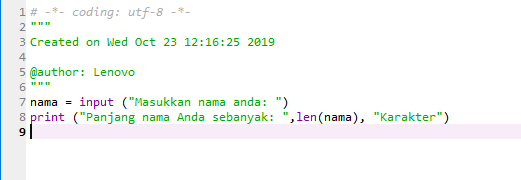
\includegraphics[width=9cm]{input/inp1.png}
	\centering
	\end{figure}
	

	\item maka akan menghasilkan output seperti berikut
	\begin{figure} [h]
	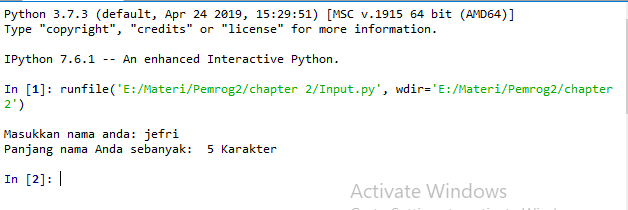
\includegraphics[width=9cm]{input/inp2.png}
	\centering
	\end{figure}
	
	
\end{enumerate}